\chapter{Introduction}
\section{Motivation}
	This work is focused on exploring the synergy between two science fields, which are outstanding nowadays: \textit{robotics} and \textit{deep learning}. These are combined for obtaining a robust system capable of following a certain person navigating towards it on a reactive behavioral. This behavioral is composed of two main components: the \textit{perception block}, responsible of processing the images from an RGB-D sensor placed on the system, and the \textit{actuation block}, which moves the robotic base accordingly to the relative position of the person to be followed.\\
	
	The original idea was proposed on \cite{tfg}, where a neural following system was developed to be run in a standard laptop into which the camera and the robot were plugged. In the following dissertation, we will revisit this work and describe the points of interest which have allowed to enhance the previous version of this work.\\
	
	The key aspects of this project can be brought in as follows:
	\begin{description}
		\item[Embedded solution] the system is mounted on a battery-powered robot, on a \textit{mobile base} form factor. This robot features a high-performance GPU embedded on a System-on-Module. Thus, this ensemble can work on its own, without requiring an external computer to perform the inferences or running algorithms in parallel. A remote monitoring of the behavioral is available as well, but it is not required for the system to work.

		\item[Person identification] the proposed system runs 3 neural networks. These networks perform inferences over the images perceived by the RGB-D sensor, which is attached to the system as the \textit{point-of-view} of the robot. The inferences are devoted to detect the different persons present in the scene, as well as to distinguish them by means of an distinguishing feature: their face.

		\item[Tracking] the full system includes a probabilistic tracker, based on dynamic modeling. This leverages the \textit{trajectories} followed by the persons while they wander on the visual field of the robot, as well as the relative distance to the person, obtained by the depth sensor included in the camera. As a result, we can have a gain on the robustness of the system, compared to a version governed exclusively by the neural inferences, which are sensitive to visual occlusions. Trusting just on these inferences could easily result on an unsteady behavioral. However, this can be avoided introducing the probabilistic modeling, as it will be explained later.
	\end{description}
	
	%	Este proyecto describe el proceso de desarrollo del sistema enunciado en el título, que condensa los puntos clave que conforman la novedad con la que justificamos el mismo:
	%- Embedded, ya que está compuesto de un robot alimentado por una batería, que soporta una placa portátil de desarrollo. Esta placa implementa algoritmos de manera totalmente local, ofreciendo una monitorización inalámbrica del funcionamiento del sistema.
	%- Person identification, combinamos de manera secuencial 3 redes neuronales que realizan inferencias sobre las imágenes percibidas por la cámara RGB-D incorporada en el robot. Este sistema combinado permite detectar a las diferentes personas presentes en la escena, así como discernir entre estas mediante un signo de identidad como es la cara.
	%- Tracking, ya que incorpora un seguimiento probabilístico basado en sistemas dinámicos. Esto se aprovecha de las trayectorias que mantienen las personas al moverse por el campo visual del robot, así como de la distancia relativa del robot a cada una de estas, gracias al sensor óptico de profundidad incorporado. Este sistema provee una robustez extra del sistema frente a posibles pérdidas totales o parciales de la persona, ante las cuales las inferencias neuronales no serían suficientes para mantener un control estable sobre el robot.
	
	
\section{State of the art}
\label{sec:1_sota}
	As it was previously introduced, this work is performed to explore the synergies on robotics and deep learning. In this section, the current approaches and tools will be studied in order to outline a general framework where this work can be placed.\\
	
	The problem to be addressed is to \textit{get a robot to follow a person}. This problem can be split into several steps, where different approaches have been previously developed. The steps will be covered in the following subsections.
	
\subsection{Person detection}
Last decades have come linked to strong advances in the computer vision field. This has vastly reduced the production prices of digital cameras and high-resolution sensors, which have come into the consumer market segment: nowadays, everybody carries at least 2 cameras in their mobile phone. This, besides an increase in the hardware performance has resulted in a strong impulse into computer vision research. There are many application possibilities using cameras, however the \textit{person detection} challenge is a recurrent one.\\

\begin{figure}[h]
	\centering
	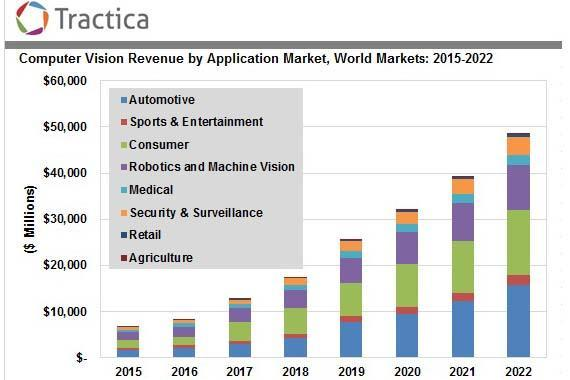
\includegraphics[width=10cm]{cv_forecast_2022}
	\caption{Computer Vision revenues in the last year, and forecast for 2022 (source: \cite{cv_forecast}).}
	\label{fig:1_cv_forecast}
\end{figure}

One of the mostly used approaches is commonly called the \textit{Viola-Jones} detector \cite{violajones}. This algorithm relies on a \textit{rigid body model}, which fits a specific shape. On a grayscale image, this shape can be typically distinguished by means of the pixel intensity levels. A spatial filters called \textit{Haar features} (\autoref{fig:1_haarfeats}) are introduced: these are used across the image looking for the intensity pattern for each mask, which should resemble a part of the rigid body. As this presents a weak decision by itself, several filters (previously chosen in a training process) are combined on a \textit{boosted cascade}. A person is detected if the weighted combination of several filters are triggered inside a certain area, which is decided to potentially contain a person \cite{diapos_cv_clasif}.

\begin{figure}[h]
	\centering
	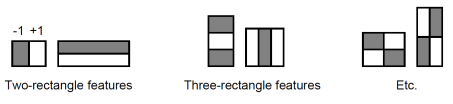
\includegraphics[width=0.7\linewidth]{haar_feats}
	\caption{Haar features: some examples \cite{diapos_cv_clasif}.}
	\label{fig:1_haarfeats}
\end{figure}

\begin{figure}[h]
	\centering
	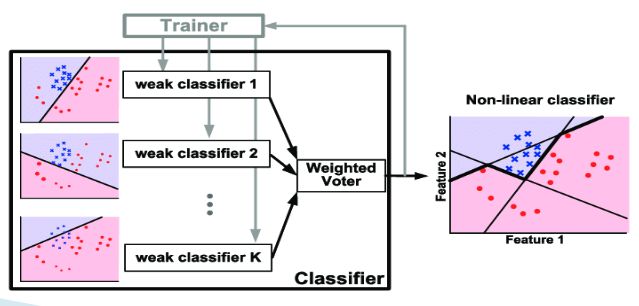
\includegraphics[width=0.7\linewidth]{boosted_cascade}
	\caption{Boosted weak classifiers \cite{diapos_cv_clasif}.}
	\label{fig:1_violajones_boost}
\end{figure}

Although this system was originally developed to detect faces, the rigid body model allows a generalization powerful enough to extend this to another object classes, \textit{person} among these. The open-source standard image processing library, OpenCV, includes pre-trained models\footnote{\url{https://github.com/opencv/opencv/blob/master/data/haarcascades}}, which can be directly used in their Viola-Jones implementation. Scale invariance can be achieved evaluating the image at multiple scales on runtime.


Another common approach nowadays for person detection is based on HoG (\textit{Histograms of Gradients}) \cite{hog_detection}. This method computes local features by means of the intensity gradients across the image, and quantizes them using their angle (creating a histogram for the oriented gradients for that pixel), as it can be seen on \autoref{fig:1_hog_sift}.\\


\begin{figure}[h]
	\centering
	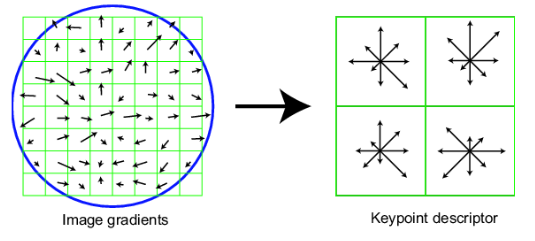
\includegraphics[width=0.7\linewidth]{hog_sift}
	\caption{Example of a HoG, quantized to 8 directions \cite{diapos_cv_features}.}
	\label{fig:1_hog_sift}
\end{figure}



These gradients are collected in $64 \times 128$ windows, and treated as features from which a linear SVM (\textit{Support Vector Machine}) is trained in order to classify a region as \textit{person/non-person}. \autoref{fig:1_hog_avg} shows the average gradient patch for a person (the direction of each gradient is not shown). A visual inspection immediately resembles the shape of a person standing up. Thus, this detector will yield the best performance when the person to be detected stands in that specific pose.

\begin{figure}[h]
	\centering
	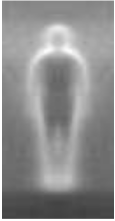
\includegraphics[width=3cm]{hog_avg}
	\caption{Average gradient for person detection on \cite{hog_detection}.}
	\label{fig:1_hog_avg}
\end{figure}

These methods, among several more approaches, have been the state-of-the-art techniques: the cornerstone are the image gradients, which can be computed with a high efficiency and present decent performance. However, their main drawback is the \textit{generalization} capability, as a successful detection is highly dependent on the person pose. However, in the latest advances, the detection frameworks have moved towards the spreading framework: \textit{deep learning}, especially the most salient tools on image processing: CNNs (\textit{convolutional neural networks}). The first steps on this field \cite{rcnn} required for a previous step on the image called \textit{region proposal}. This step is devoted to find potential regions on the image to contain an object. This way, the challenge was to label these region according to the objects contained inside, reducing the problem to a classification task. However, the process to find these undetermined regions and iterate over them makes the process too slow for real-time requirements, which are explicitly contained in our objectives. Care has been put in posterior works \cite{fastrcnn} \cite{spp} to reduce this computation time. However, this reduction in time brings about a reduction in precision as well.\\


On the other hand, one of the most remarkable architectures is SSD (\textit{Single-Shot Multibox Detector}) \cite{ssd}. The main benefit from this architecture is the fact that it embeds all the required computations in a single neural network, reducing the complexity compared to other approaches requiring external region proposals, as it was depicted above. This greatly reduces the computational time when the network has to evaluate an image. As it was depicted in \cite{tfg}, the architecture is split into stages:\\

% ============================================================================

\begin{description}
	
	\item[Reshape] the posterior stages evaluate the image on a fixed tensor size of $n \times 300 \times 300 \times 3$ (being $n$ the size of the input batch). Other image sizes might be used, however this one offers a good trade-off between score and computational load.
	
	\item [Base network] this first group of layers are reused from a typical image classification model, such as VGG-16 \cite{vgg16}. The first layer from this architecture are utilized in this design, truncated before the first classification layer. This way, the network can leverage the \textit{feature maps} from the classification network, in order to find objects inside the input image. At the output of this network, several convolutional layers are appended, decreasing in size. This has the objective of predict detections at multiple scales. One thing to mention at this point is that the base network can be a different one rather than VGG-16, such as a MobileNet \cite{mobilenet}, which is highly optimized for running on low specifications devices. This is interesting as our embedded system will be limited in computing power, thus it will be revisited in future sections.
	
	\item[Box predictors] later, for each extracted set, a dedicated operation is performed, generating a small set (typically 3 or 4) fixed-size \textit{anchors}, with varying aspect ratios for each cell on a grid over the activation map (\autoref{fig:5_ssd_generated_boxes}). As these maps have different sizes, this aims to detect  objects in different scales. The anchors are then convolved with small filters (one per depth channel), which output \emph{softmaxed confidence values for each known class}, and \emph{offsets/adjustments for the generated bounding box}. So, for each detected object (on that scale), we know the score for each class and its estimated position inside the feature map (hence, in the image as well).
	
	\item \emph{Postprocessor}: as several detections might be triggered in the same area for different classes and scales, a \textit{Non-Maximum-Supression} operation is performed at the output of the network to retain the boxes with a larger area.
\end{description}
	\begin{figure}[h]
	\centering
	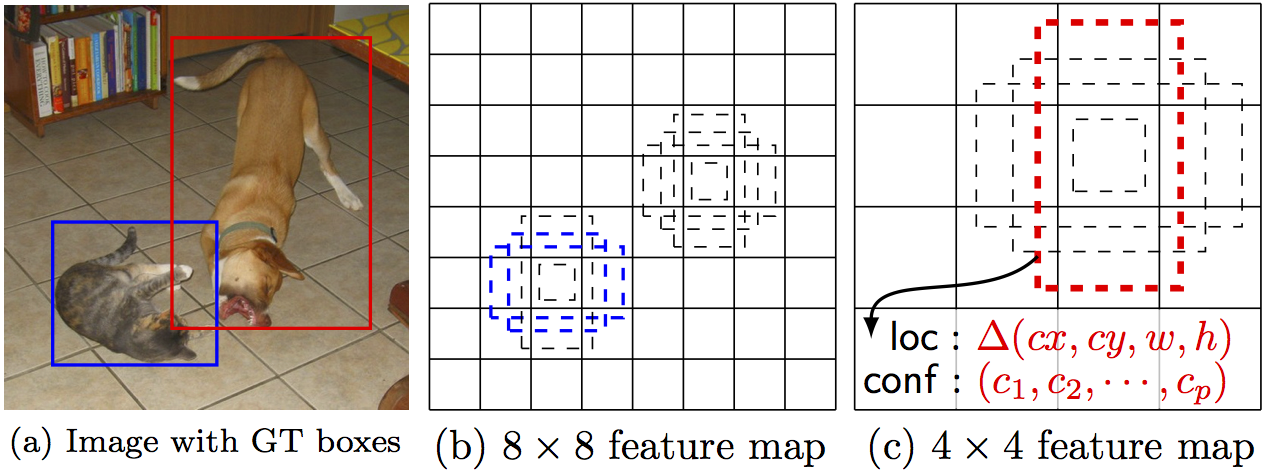
\includegraphics[width=0.7\linewidth]{ssd_generated_boxes}
	\caption{A set of boxes are generated centered on each point of every feature map \cite{ssd}.}
	\label{fig:5_ssd_generated_boxes}
\end{figure}


Another interesting approach on the neural networks field is the YOLO (\textit{You Only Look Once}) system \cite{yolov1}, which has been iteratively revised in two occasions so far \cite{yolov2} \cite{yolov3}.

The latest implementation, YOLOv3 \cite{yolov3} features residual networks \cite{resnets}, which tackle the problem of \textit{vanishing gradients} when the networks become deeper. The stacking of several layers results on gradients diminishing its value up to a point the precision mode of the machine is not able to handle. The gradients are canceled, burdening the training process, as the first layers parameters take a substantially higher time to converge. The residual networks added in this revision of the design add shortcut connections across the layers, centering the backpropagation gradients on 1. As the publication says \cite{yolov3}, the combination of these residual layers and convolutional ones allows to train much deeper architectures, capable of yielding a higher generalization. As in the SSD detectors, the YOLO architecture performs multi-scale detections, using 3 scales for splitting the feature maps into cell grids. On each of these cells, 3 anchor bounding boxes are fit. These anchors are selected by running the k-means algorithm on the COCO datasets selecting 9 clusters (3 anchor shapes $\times$ 3 scales). This aims to a better generalization as well, as in the R-CNN \cite{rcnn} and the SSD \cite{ssd} the anchor shapes are hand-picked.\\

For each (anchor, cell, scale) combination, this network predicts:

\begin{itemize}
	\item The coordinates of the object inside the anchor. Details can be visualized on \autoref{fig:1_yolo_output}.
	
	\item \textit{objectness} score, which is computed by means of a logistic regression in order to determine the probability of overlap with a ground truth bounding box more than any other prior anchor.
	
	\item 80 scores, as the original implementation is trained in the COCO dataset, which contains 80 classes. These classes might be overlapping (e.g. ``woman" and ``person"). Thus, these scores are computed by independent logistic classifiers and are not passed through a \textit{softmax} operation.
\end{itemize}


\begin{figure}[h]
	\centering
	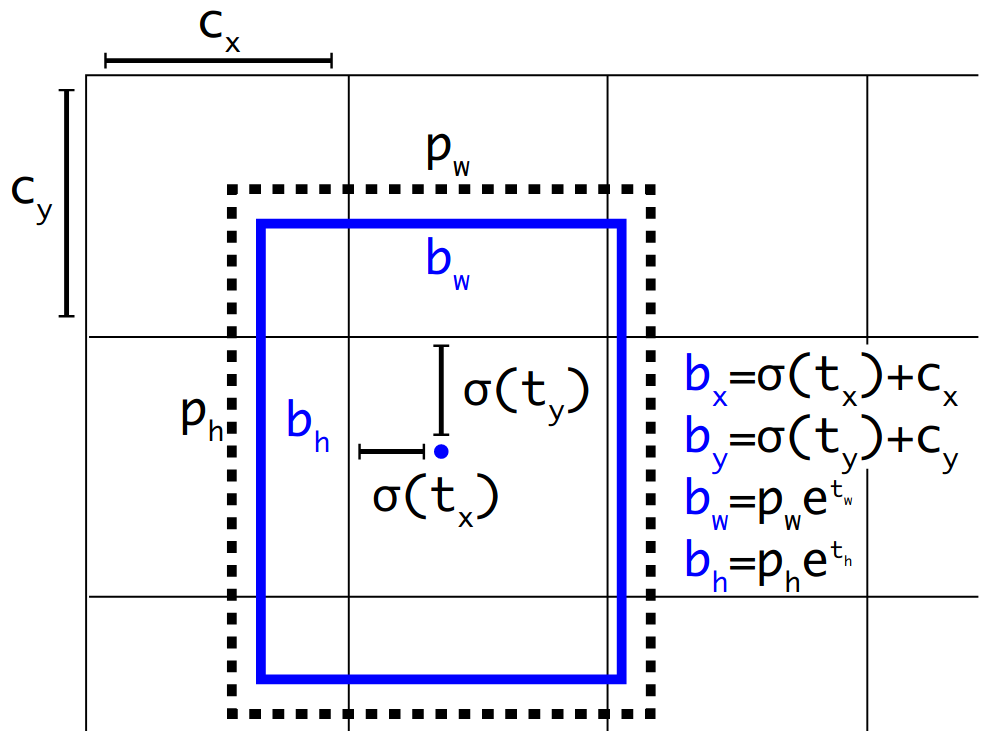
\includegraphics[width=0.5\linewidth]{yolo_outputs}
	\caption{Output on YOLO for each anchor and cell. The dashed line represents the prior anchor, while the blue line represents the detection which corrects that anchor.}
	\label{fig:1_yolo_output}
\end{figure}

\subsection{Person identification}
On a controlled environment, where the only present person is the one to be followed, a person detection system could be enough for following purposes. However, in a normal scenario, there might be several people inside the field of vision of the robot. This problem can be approached by means of adistinguishing feature of the person of interest, provided beforehand. One example is \cite{color_id}, which computes the color distribution of the person of interest, and later compares this distribution with the ones belonging to the different persons using the Bhattacharyya coefficient, which is designed to measure the similarity between the color histograms of the reference person and the detected one. However, this system can be deceived replicating the color distribution of the person of interest: wearing similar clothes helps to reduce the distance between the histogram, leaving a chance to confound another person with the one to follow.\\

A more robust approach is to use the \textit{face} of the person as the distinguishing feature, as its uniqueness makes it a good reference to identify the detected person. Several approaches \cite{dlib_review} extract facial \textit{landmarks} from the morphology of a given face, and use them to classify the face, comparing it against a set of known faces and predicting the identity based on the distance to each known face. Some open-source libraries such as \texttt{dlib} and \texttt{OpenCV} provide the algorithms to perform these processes.\\

\begin{figure}[h]
	\centering
	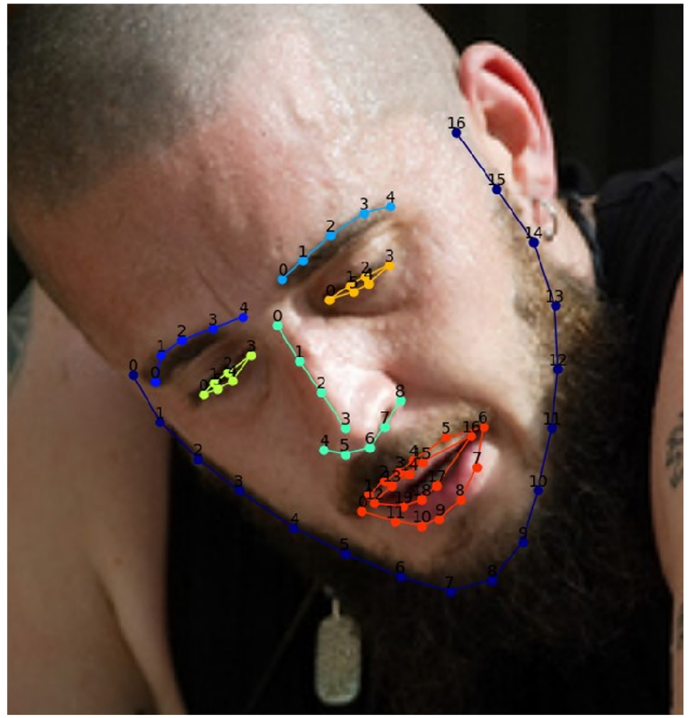
\includegraphics[width=0.6\linewidth]{dlib_landmarks}
	\caption{Facial landmarks are dependent of the face shape and morphology (image from \cite{dlib_review}).}
	\label{fig:1_dlib_landmarks}
\end{figure}


The intuition behind these methods are to \textit{project} the image of the face into a lower dimensional space, which allows to extract significant features from each face. These features have to be consistent for the same face across different pose and lighting conditions (\autoref{fig:1_faces_poses}). An useful transformation when a dimensionality reduction is pursued is PCA (\textit{Principal Component Analysis}), a linear transformation that can be implemented to deal with the face recognition problem \cite{face_pca}.

\begin{figure}[h]
	\centering
	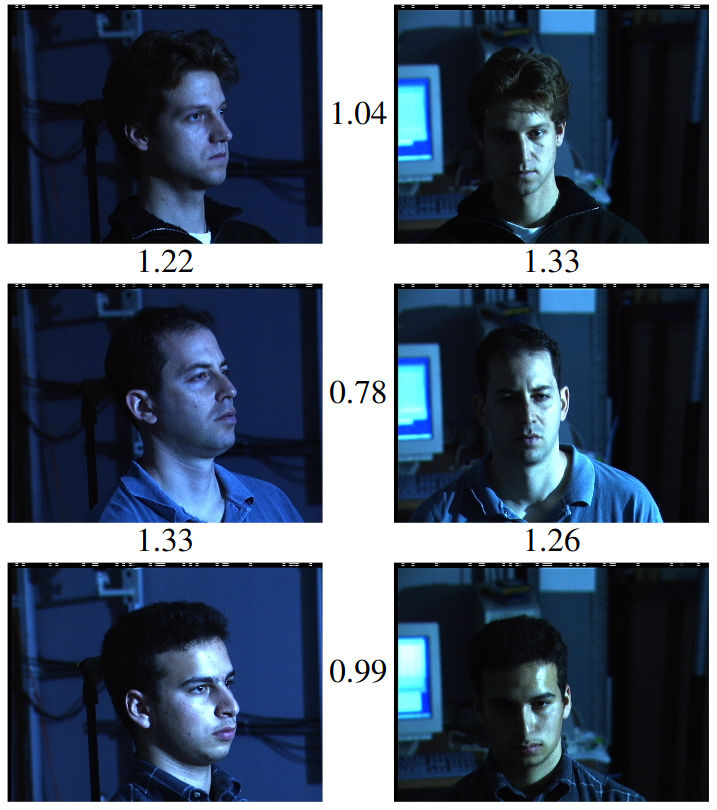
\includegraphics[width=0.5\linewidth]{face_poses}
	\caption{Examples of poses and light conditions across which the face projections are desired to be consistent for the same person (image from \cite{facenet}).}
	\label{fig:1_faces_poses}
\end{figure}


However, once again neural networks can be leveraged in order to achieve this and more: as the PCA is a linear operation, it could be learned by a single layer neural network. Thus, the introduction of deep networks can yield interesting results. The most relevant approach so far uses deep convolutional networks for performing this process \cite{facenet}, implementing an architecture called \textit{FaceNet}, which is partially based on the Inception \cite{inception} module, designed by Google researchers in order to greatly reduce the number of parameters in a neural network. What this network computes is called an \textit{embedding}, a projection of the input face image into a point in a 128-dimensional hypersphere. This allows to translate the identification into linear algebra terms, such as \textit{distance} between two faces, clustering and applying unsupervised algorithms in order to determine the identity of a trivial face, among a collection of known regions. These networks can be trained using a loss function  called \textit{triplet loss}, inspired by the work in \cite{lmnn_loss}. Given a training sample (\textit{anchor}), a \textit{positive} example (same class than the anchor) and a \textit{negative} example (different class than the anchor) are chosen, and the network is tuned to maximize the \textit{anchor-negative} embeddings distance, and minimize at the same time the \textit{anchor-positive} one (\autoref{fig:1_facenet_triplet_loss}).

\begin{figure}[h]
	\centering
	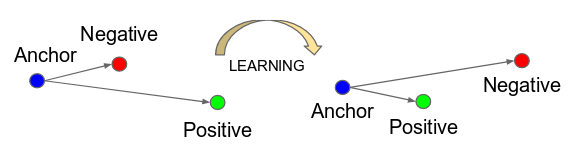
\includegraphics[width=0.7\linewidth]{facenet_triplet_loss}
	\caption{Triplet loss training. It minimizes the distance between an \emph{anchor} (current example) and a \emph{positive}, both of which have the same identity, and maximizes the distance between the \emph{anchor} and a \emph{negative} of a different identity (from \cite{facenet}).}
	\label{fig:1_facenet_triplet_loss}
\end{figure}


One thing to mention about the algorithms described above is that they perform the operations on the image of a face. Thus, a face detection system is required for previously cropping the face of the person to be identified. Once again, a neural approach can be reduced to an \textit{object detection} problem (detecting the class \textit{face}, in this case). One interesting approach using this technique is \textit{faced} \cite{faced}. This is a custom small ensemble of two neural networks, responsible to detect faces and correct the bounding boxes found. The main objective of the system is \textit{speed}, so the main detector architecture is based in YOLO \cite{yolov1}, and the second correction stage raises the precision achieved by the detector.

\begin{figure}[h]
	\centering
	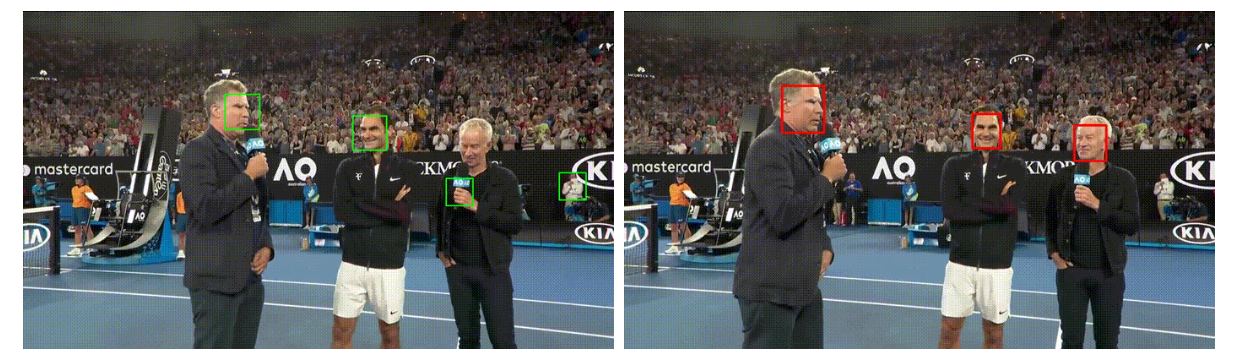
\includegraphics[width=0.8\linewidth]{faced_vs_haar}
	\caption{Classical Haar based face detector \cite{violajones} (left) vs. \textit{faced} (right). Image from \cite{faced}.}
	\label{fig:1_faced_vs_haar}
\end{figure}


%\subsection{Person tracking}

\subsection{Embedded deployment}
One of the requirements of this work is to be integrated in an autonomous system. This imposes a power limitation on the algorithms to be deployed. Generally, the robotic systems are deployed using laptops connected to robots, at it was done in \cite{tfg}.

\begin{figure}[h]
	\centering
	\begin{subfigure}[h]{0.4\linewidth}
		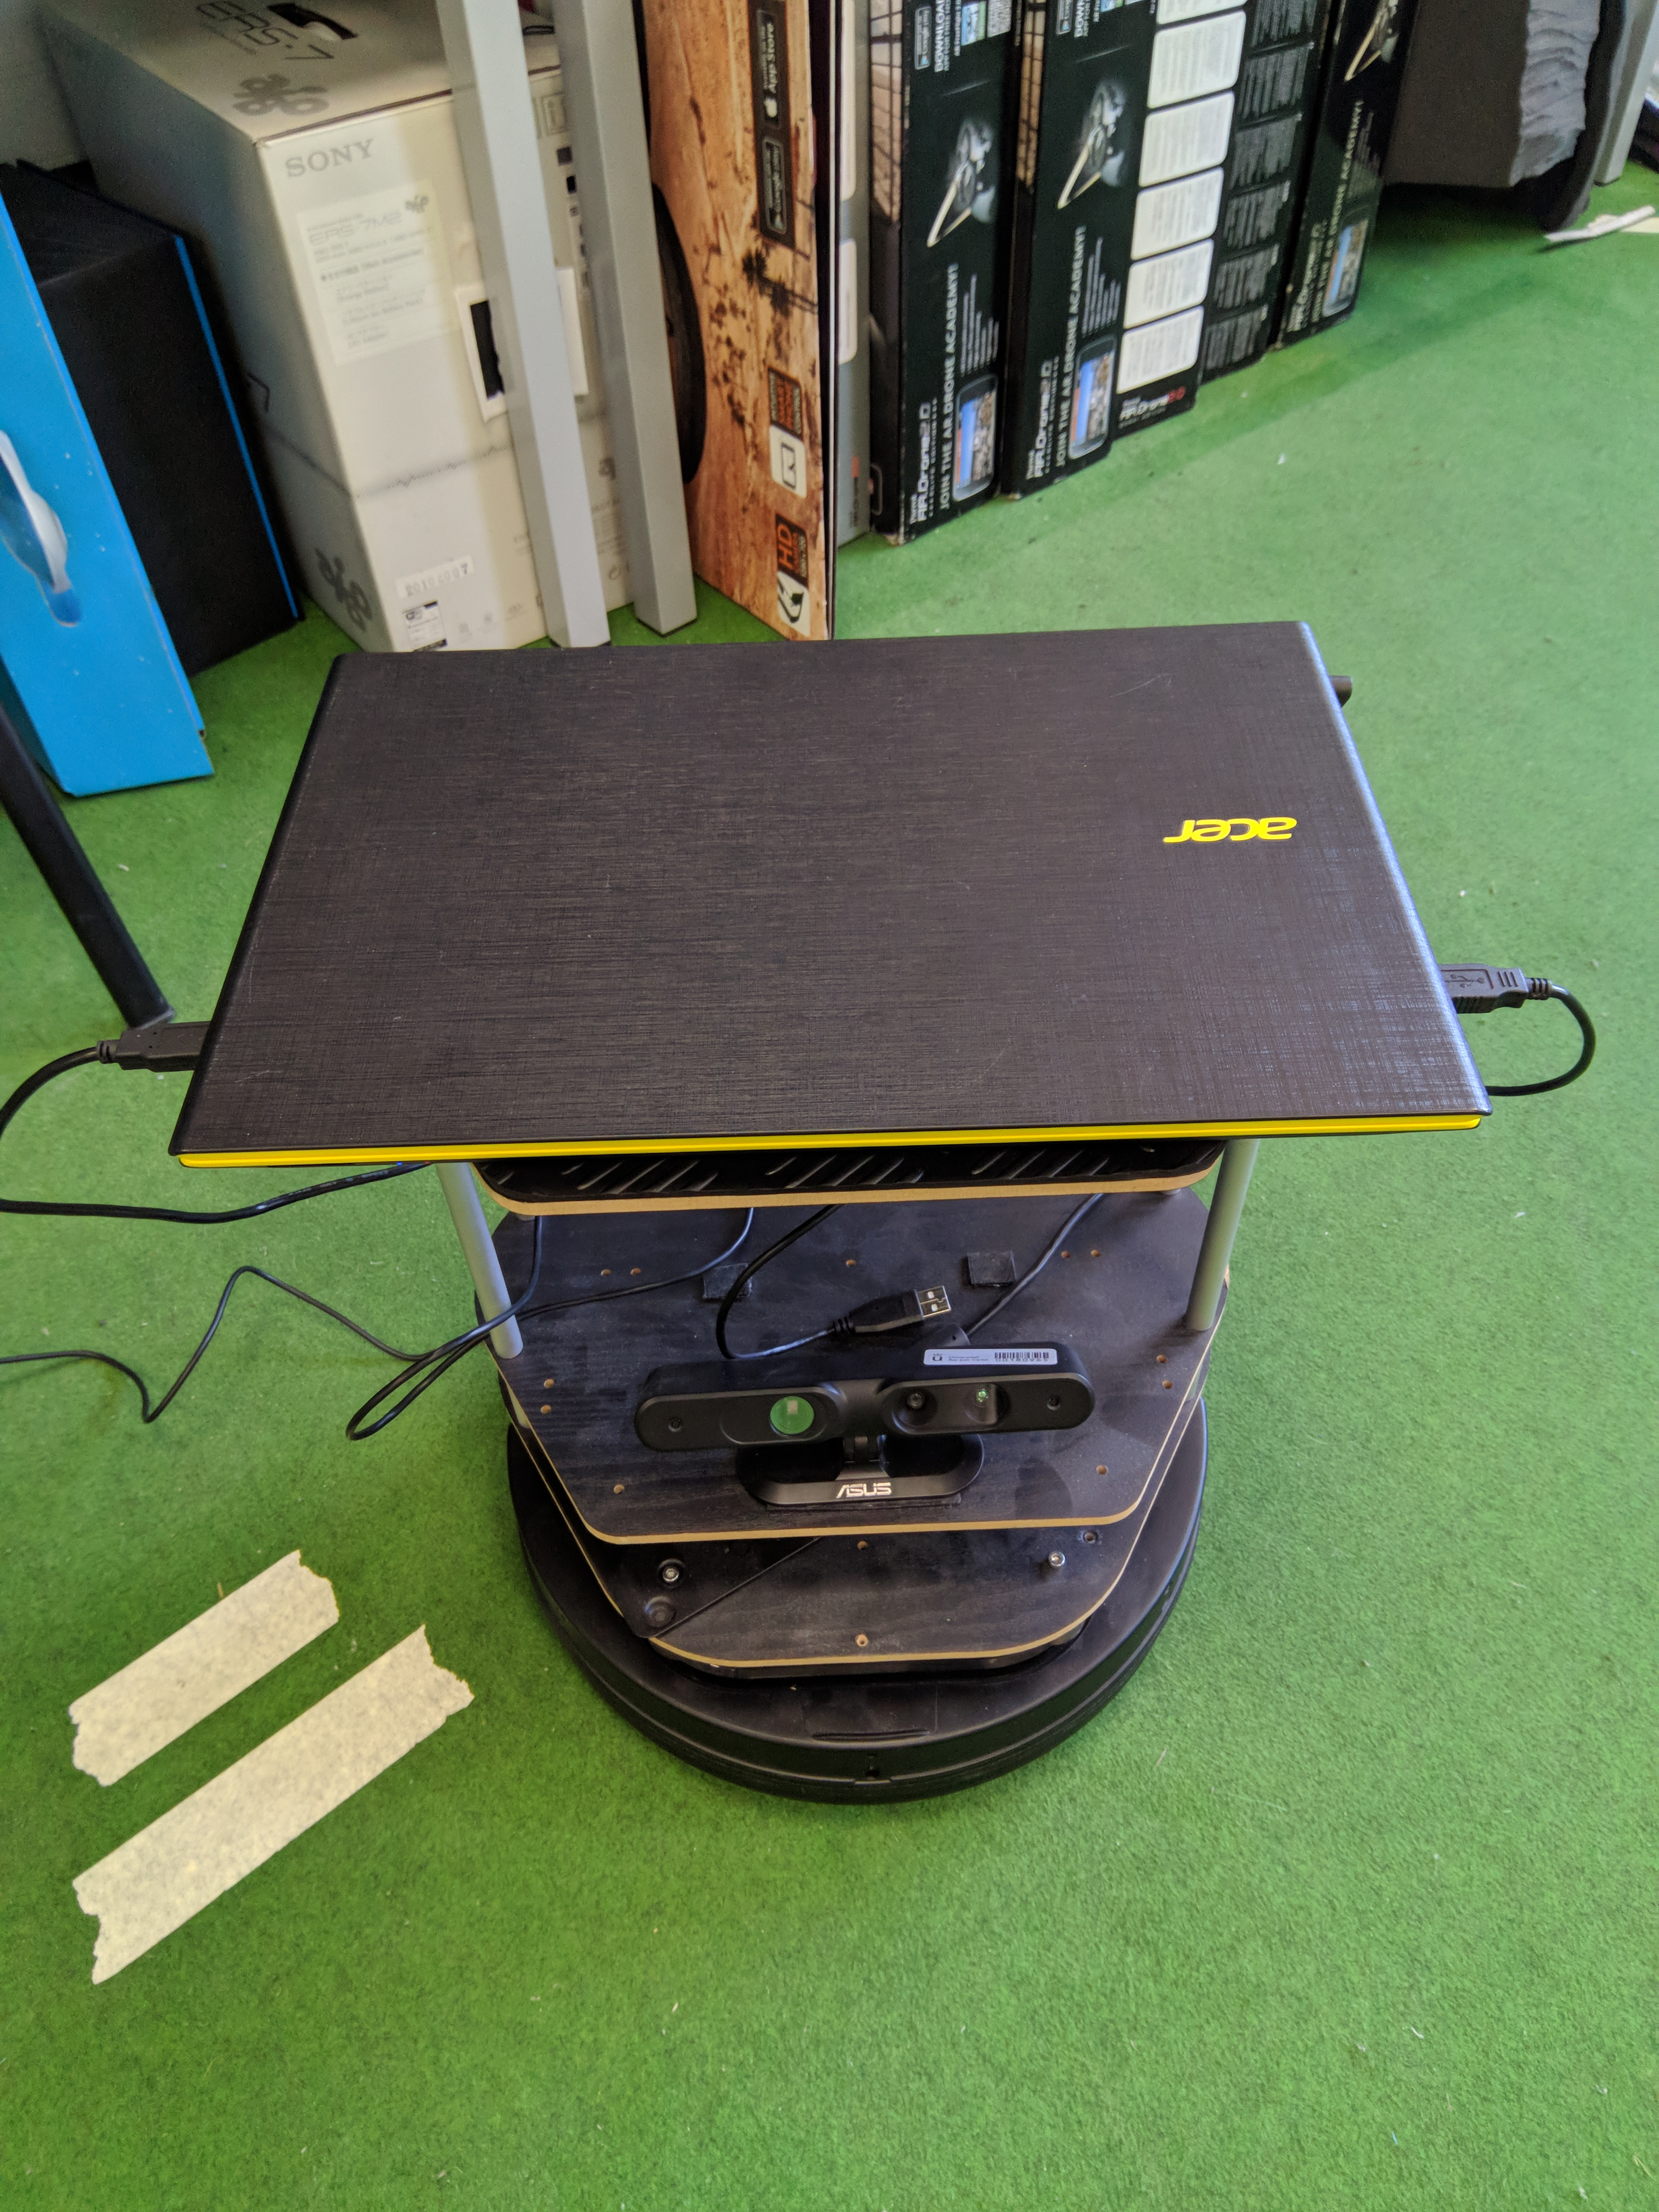
\includegraphics[width=1.9in]{tfg1}
		\caption{Frontal view.}
		\label{fig:3_turtlebot_front}
	\end{subfigure}
	\begin{subfigure}[h]{0.4\linewidth}
		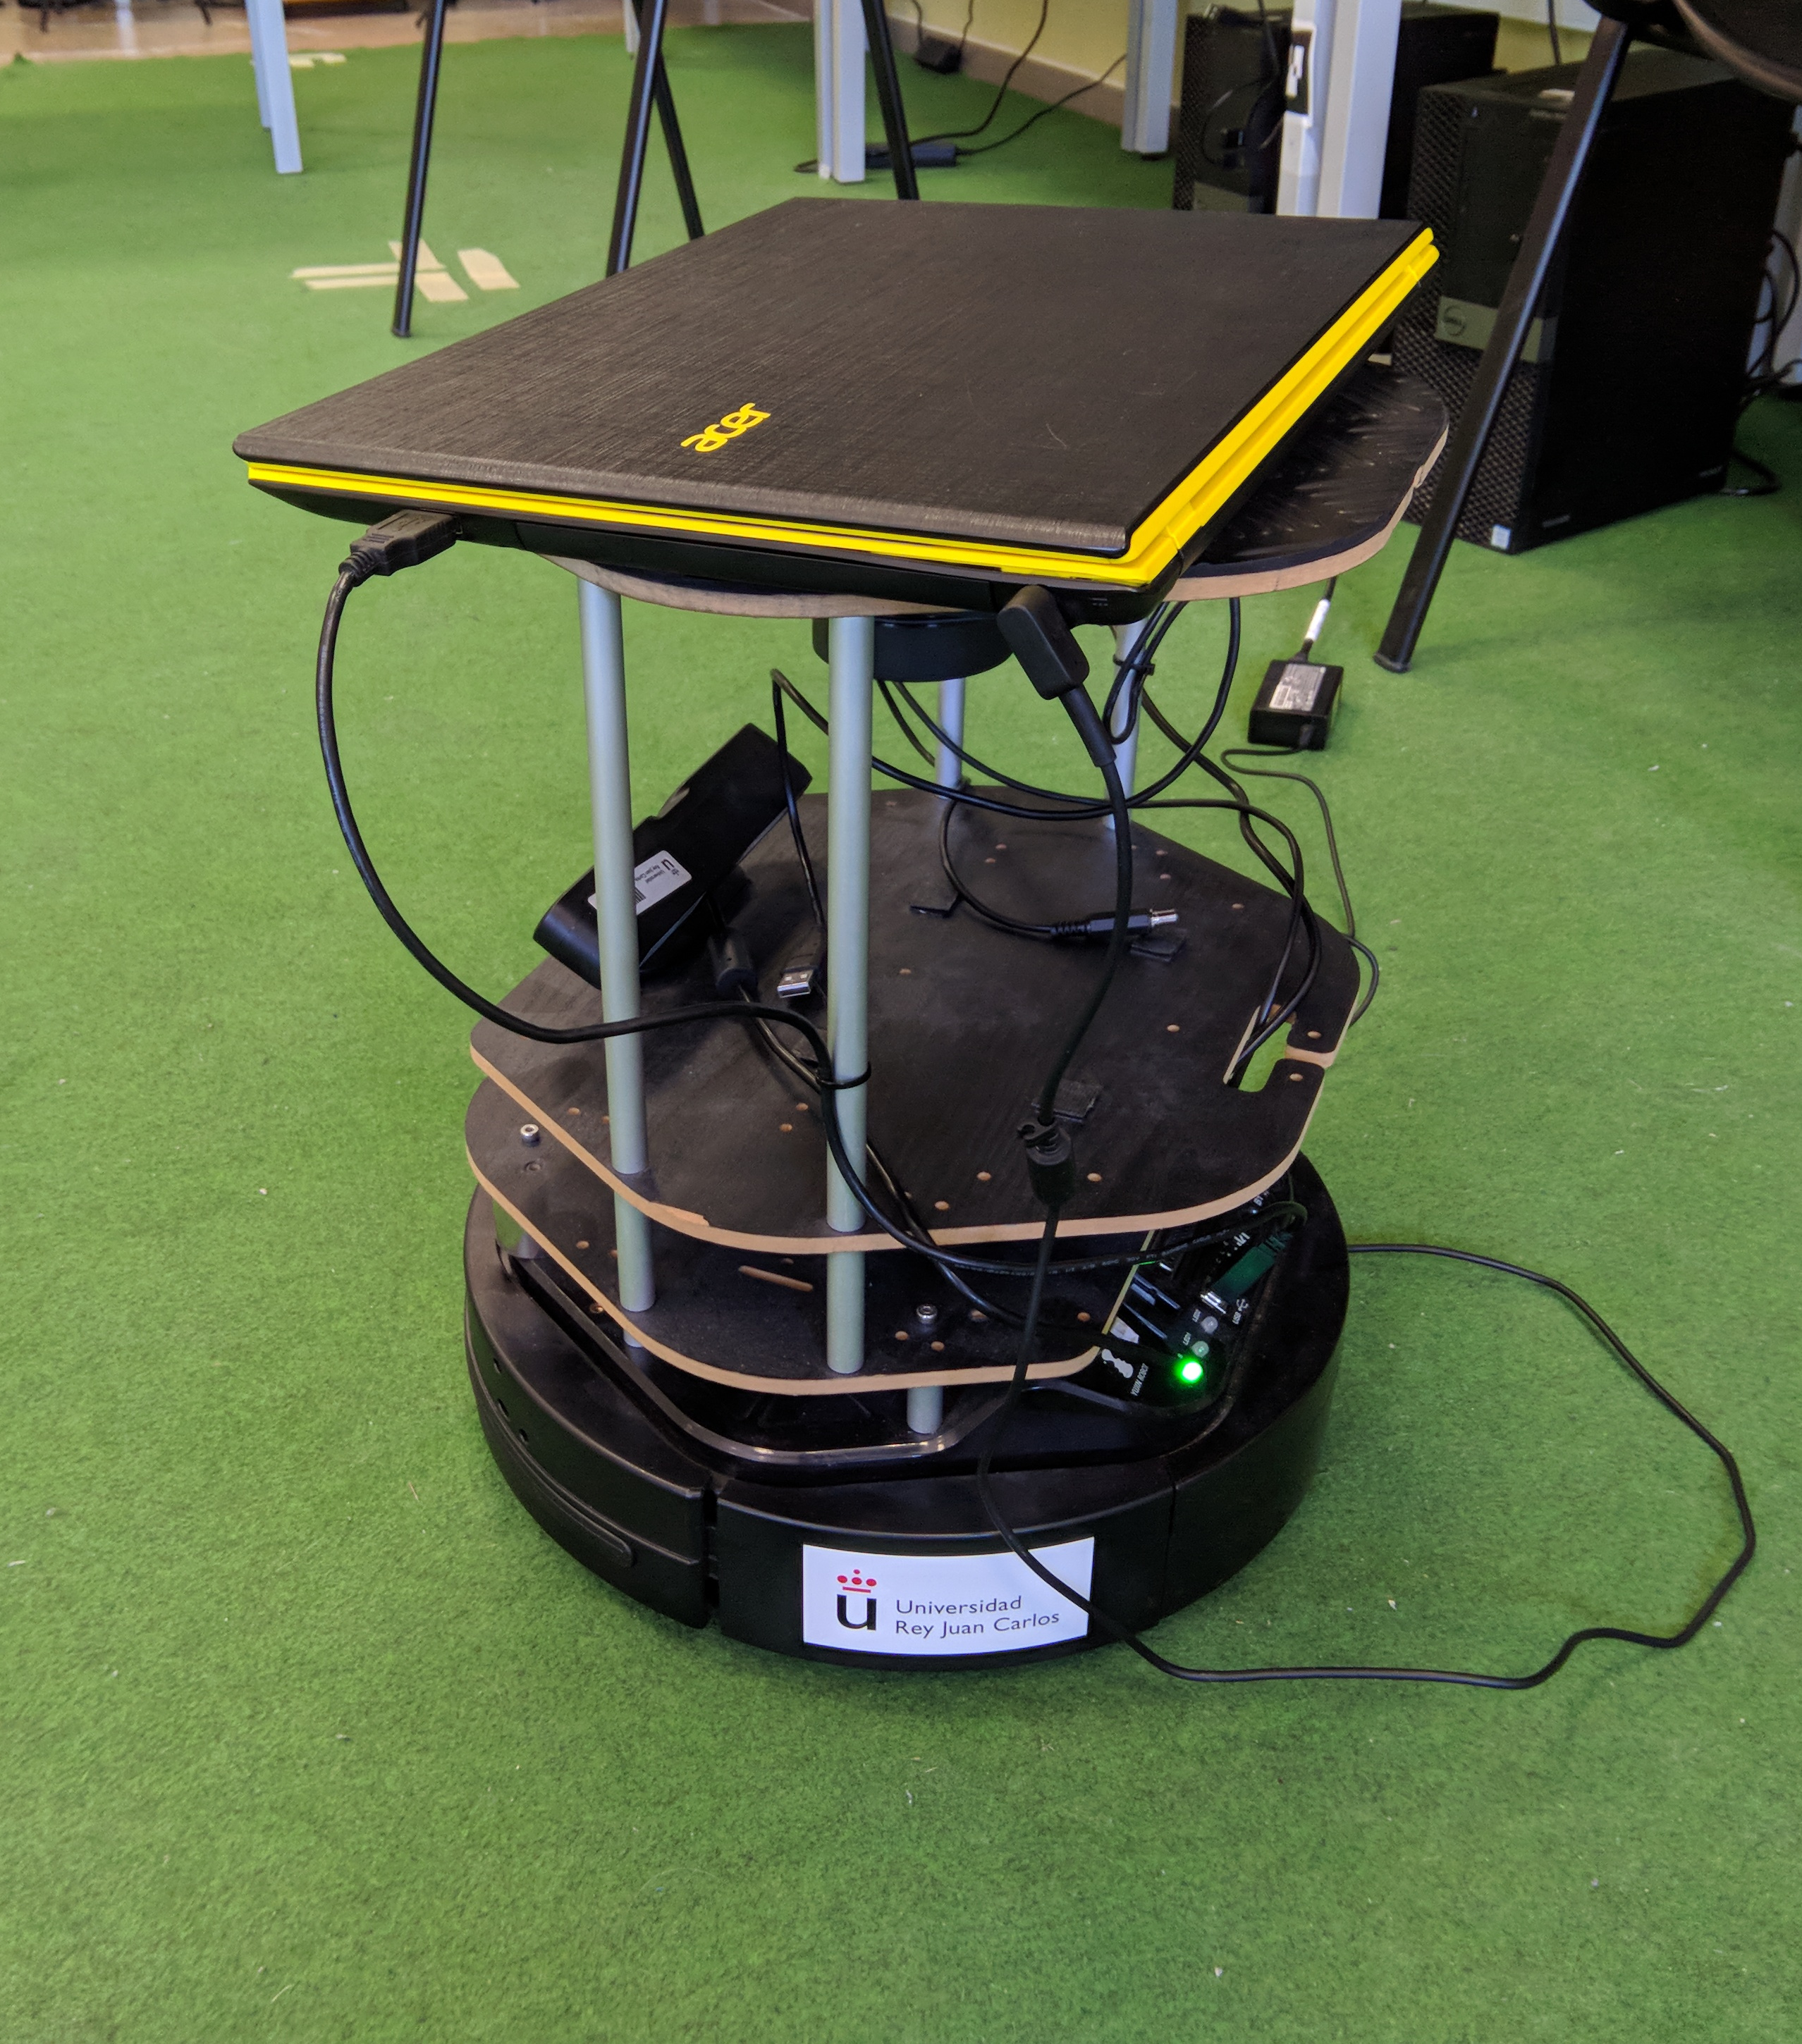
\includegraphics[width=2.2in]{tfg2}
		\caption{Side view.}
		\label{fig:3_turtlebot_side}
	\end{subfigure}
	\caption{Laptop+robot deployment on \cite{tfg}.}
	\label{fig:1_real_tfg}
\end{figure}

Nowadays, the mentioned increase in the interest into the real-time computer vision applications has fostered the development of specific low-power embedded devices to be integrated in mobile systems. The extending usage of devices such as Arduino or Raspberry Pi has led to embedded robotics systems, such as PiBot \cite{pibot} (\autoref{fig:1_pibot}). These robots are useful in the educational scope, as they are capable of running simple vision and navigation algorithms at a low cost.
\begin{figure}[h]
	\centering
	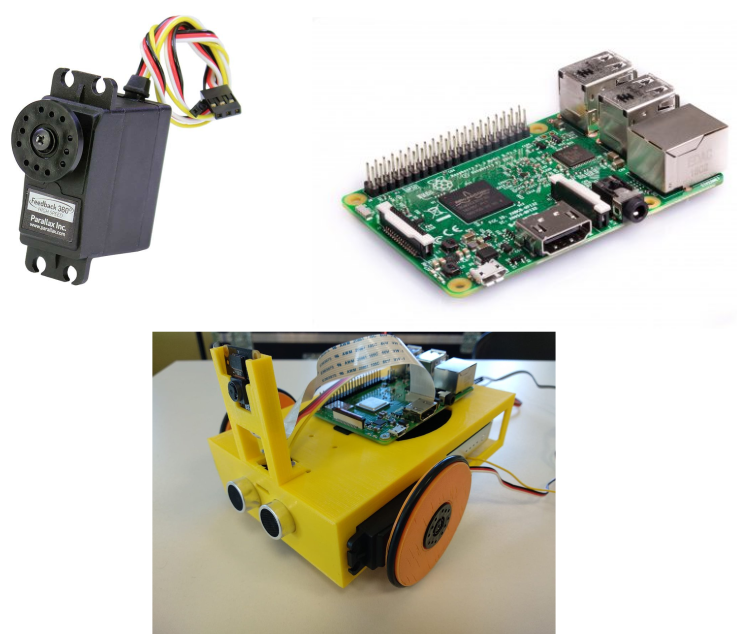
\includegraphics[width=0.5\linewidth]{pibot}
	\caption{PiBot, an open low-cost robotic platform for education (image from \cite{pibot}).}
	\label{fig:1_pibot}
\end{figure}
Unfortunately, the requirements on systems running more complex algorithms, such as neural networks, require of the next tier in power terms, keeping the portability nevertheless. The ideal device could be an ASIC, as the custom design would lead to a very tight optimization of the performance. However, we are aiming to run the algorithms on existing software frameworks, so we aim to general purpose computers instead. The most remarkable advance in this scope are the Jetson devices manufactured by NVIDIA. These development boards are SoM (\textit{System-on-Module}) computers running a tailored version of Linux. The fundamental feature of these systems is that they include a high-performance GPU featuring CUDA, a low-level parallel computation library, as well as several toolkits designed to optimize as much as possible the software implementations for the plethora of possibilities to be designed on this board. As it can be seen in \autoref{fig:1_tx2}, its size and power consumption make of this system a good choice to be included in an autonomous robotic system. 
\begin{figure}[h]
	\begin{subfigure}[h]{0.45\linewidth}
		\centering
		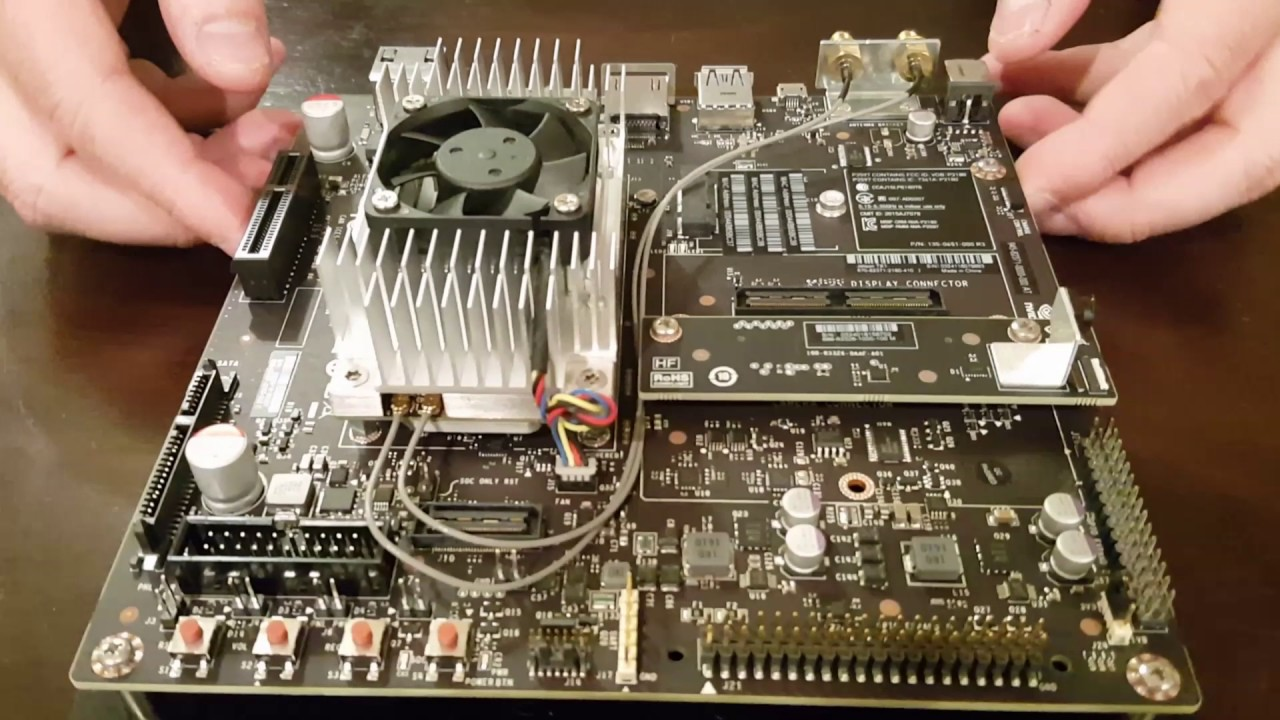
\includegraphics[width=\linewidth]{jetsontx2}

	\end{subfigure}
	\begin{subfigure}[h]{0.45\linewidth}
		\centering
		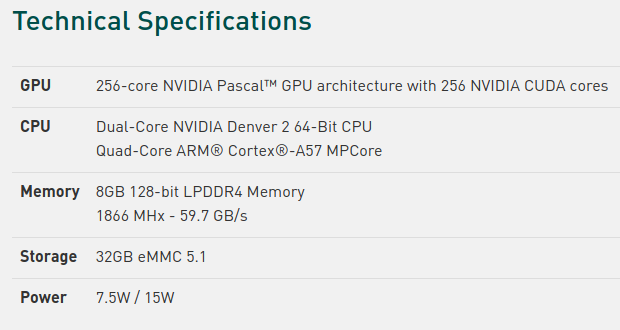
\includegraphics[width=\linewidth]{tx2_specs}
	\end{subfigure}
	\caption{NVIDIA Jetson TX2: an embedded high-performance device including a GPU.}
	\label{fig:1_tx2}
\end{figure}


\subsection{Person following}
Several approaches have been developing pursuing this challenge of \textit{following a person}. Once the perception algorithms are established, the final output of the pipeline has to be a movement command for the robot to move towards the desired point. Mobile  robots can be classified according to their locomotion capabilities. A good summary can be that a robot is \textit{holonomic} if the number of its controllable degrees of freedom is equal to its total degrees of freedom. If the controllable degrees of freedom are lower than the total degrees of freedom, the robot is \textit{non-holonomic}.\\

In the case of a holonomic robot, the navigation process is simplified, as the robot can instantaneously move to a desired target. However, a non-holonomic robot needs to perform maneuvers in order to move towards a point.\\

\section{Objectives}
\label{sec:1_objectives}
	This work has been carried out in order to fulfill certain requirements in a particular person following application:
	
	\begin{enumerate}
		\item Achieve a real-time following behavioral using embedded low-power hardware and a low-complexity educational robot.
		
		\item Build the inference pipeline using exclusively concurrent CNNs (\textit{convolutional neural networks}).
		
		\item Combine a neural system with probabilistic filtering to carry out a robust multimodal tracking of the persons in front of the robot. This will provide the system with extra endurance and robustness against detection losses/occlusions.
	\end{enumerate}
	
These objectives allow to summarize the starting point for the development of this project: the available materials are an educational robot equipped with a battery, an embedded \textit{SoM} and a RGB-D sensor.\\

The result will be an autonomous robot which will follow a specific person, whose face has to be known beforehand (using a \textit{reference face} image).
